\subsection{Scenario 4: Unstable Infrastructure}
\textit{This scenario removes an existing infrastructure node after $30$ seconds, and adds the node back into the infrastructure after another $30$ seconds. This is repeated twice. The purpose of this scenario is to see how the system behaves when the infrastructure (connection) is unstable.}

\begin{figure}[H]
    \centering
    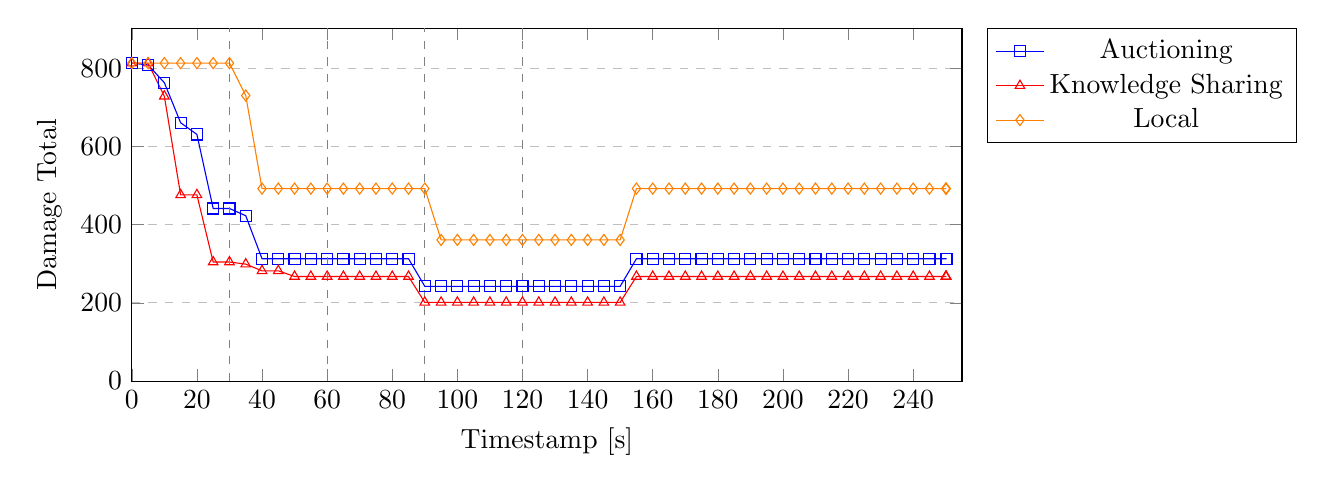
\begin{tikzpicture}
\begin{axis}[
    xlabel={Timestamp [s]},
    ylabel={Damage Total},
    xmin=0, xmax=255000,
    ymin=0, ymax=902,
    legend pos=outer north east,
    ymajorgrids=true,
    grid style=dashed,
    width=\textwidth,
    height=0.5\textwidth,
    scaled x ticks=base 10:-3,
    xtick scale label code/.code={}
]

	\addplot[color=blue,mark=square] coordinates {
        (0,812.71)(5000,808.17)(10000,762.80)(15000,660.38)(20000,630.54)(25000,441.18)(30000,441.18)(35000,422.77)(40000,312.76)(45000,312.76)(50000,312.76)(55000,312.76)(60000,312.76)(65000,312.76)(70000,312.76)(75000,312.76)(80000,312.76)(85000,312.76)(90000,242.13)(95000,242.13)(100000,242.13)(105000,242.13)(110000,242.13)(115000,242.13)(120000,242.13)(125000,242.13)(130000,242.13)(135000,242.13)(140000,242.13)(145000,242.13)(150000,242.13)(155000,312.76)(160000,312.76)(165000,312.76)(170000,312.76)(175000,312.76)(180000,312.76)(185000,312.76)(190000,312.76)(195000,312.76)(200000,312.76)(205000,312.76)(210000,312.76)(215000,312.76)(220000,312.76)(225000,312.76)(230000,312.76)(235000,312.76)(240000,312.76)(245000,312.76)(250000,312.76)(250270,312.76)
    };
    \addlegendentry{Auctioning}
	\addplot[color=red,mark=triangle] coordinates {
        (0,812.71)(5000,812.71)(10000,728.19)(15000,476.06)(20000,476.06)(25000,304.33)(30000,304.33)(35000,298.99)(40000,281.89)(45000,281.89)(50000,267.31)(55000,267.31)(60000,267.31)(65000,267.31)(70000,267.31)(75000,267.31)(80000,267.31)(85000,267.31)(90000,201.16)(95000,201.16)(100000,201.16)(105000,201.16)(110000,201.16)(115000,201.16)(120000,201.16)(125000,201.16)(130000,201.16)(135000,201.16)(140000,201.16)(145000,201.16)(150000,201.16)(155000,267.31)(160000,267.31)(165000,267.31)(170000,267.31)(175000,267.31)(180000,267.31)(185000,267.31)(190000,267.31)(195000,267.31)(200000,267.31)(205000,267.31)(210000,267.31)(215000,267.31)(220000,267.31)(225000,267.31)(230000,267.31)(235000,267.31)(240000,267.31)(245000,267.31)(250000,267.31)(250172,267.31)
    };
    \addlegendentry{Knowledge Sharing}
	\addplot[color=orange,mark=diamond] coordinates {
        (0,812.71)(5000,812.71)(10000,812.71)(15000,812.71)(20000,812.71)(25000,812.71)(30000,812.71)(35000,729.98)(40000,492.04)(45000,492.04)(50000,492.04)(55000,492.04)(60000,492.04)(65000,492.04)(70000,492.04)(75000,492.04)(80000,492.04)(85000,492.04)(90000,492.04)(95000,360.79)(100000,360.79)(105000,360.79)(110000,360.79)(115000,360.79)(120000,360.79)(125000,360.79)(130000,360.79)(135000,360.79)(140000,360.79)(145000,360.79)(150000,360.79)(155000,492.04)(160000,492.04)(165000,492.04)(170000,492.04)(175000,492.04)(180000,492.04)(185000,492.04)(190000,492.04)(195000,492.04)(200000,492.04)(205000,492.04)(210000,492.04)(215000,492.04)(220000,492.04)(225000,492.04)(230000,492.04)(235000,492.04)(240000,492.04)(245000,492.04)(250000,492.04)(250190,492.04)
    };
    \addlegendentry{Local}

	\addplot[color=gray, dashed,] coordinates {(30000,0) (30000,902)};
	\addplot[color=gray, dashed,] coordinates {(60000,0) (60000,902)};
	\addplot[color=gray, dashed,] coordinates {(90000,0) (90000,902)};
	\addplot[color=gray, dashed,] coordinates {(120000,0) (120000,902)};


\end{axis}
\end{tikzpicture}
    \caption{This graph shows the overall damage of the system in the unstable scenario. The damage is shown for each of the three strategies. The vertical lines indicate the time at which a node was removed and added again.}
    \label{fig:overall-damage-unstable}
\end{figure}

From this first Figure \ref{fig:overall-damage-unstable} we see a trend that is similar to the one from the first experiment (Figure \ref{fig:overall-damage-no-change}). The second time a node gets removed and then added, we see a small dip in the graphs. But apart from this there are no \emph{new} risks to mitigate as the properties of the nodes do not change. This is also reflected in Figure \ref{fig:messages-unstable}, where the knowledge-sharing agent does not see any property changes (and thus does not send any messages). The auctioning node does send some messages, as perviously due to the attempts of finding adaptations.

\begin{figure}[H]
    \centering
    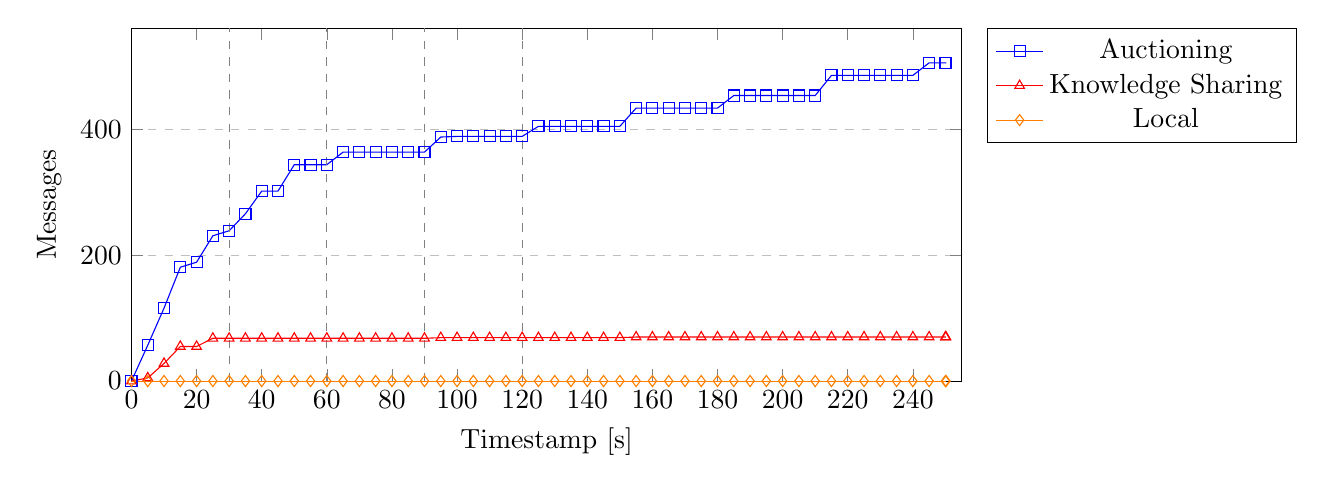
\begin{tikzpicture}
\begin{axis}[
    xlabel={Timestamp [s]},
    ylabel={Messages},
    xmin=0, xmax=255000,
    ymin=0, ymax=561,
    legend pos=outer north east,
    ymajorgrids=true,
    grid style=dashed,
    width=\textwidth,
    height=0.5\textwidth,
    scaled x ticks=base 10:-3,
    xtick scale label code/.code={}
]

	\addplot[color=blue,mark=square] coordinates {
        (0,0)(5000,57)(10000,116)(15000,181)(20000,189)(25000,231)(30000,239)(35000,266)(40000,302)(45000,302)(50000,344)(55000,344)(60000,344)(65000,364)(70000,364)(75000,364)(80000,364)(85000,364)(90000,364)(95000,388)(100000,389)(105000,389)(110000,389)(115000,389)(120000,389)(125000,405)(130000,405)(135000,405)(140000,405)(145000,405)(150000,405)(155000,434)(160000,434)(165000,434)(170000,434)(175000,434)(180000,434)(185000,454)(190000,454)(195000,454)(200000,454)(205000,454)(210000,454)(215000,486)(220000,486)(225000,486)(230000,486)(235000,486)(240000,486)(245000,506)(250000,506)(250270,506)
    };
    \addlegendentry{Auctioning}
	\addplot[color=red,mark=triangle] coordinates {
        (0,0)(5000,5)(10000,28)(15000,55)(20000,55)(25000,68)(30000,68)(35000,68)(40000,68)(45000,68)(50000,68)(55000,68)(60000,68)(65000,68)(70000,68)(75000,68)(80000,68)(85000,68)(90000,68)(95000,69)(100000,69)(105000,69)(110000,69)(115000,69)(120000,69)(125000,69)(130000,69)(135000,69)(140000,69)(145000,69)(150000,69)(155000,70)(160000,70)(165000,70)(170000,70)(175000,70)(180000,70)(185000,70)(190000,70)(195000,70)(200000,70)(205000,70)(210000,70)(215000,70)(220000,70)(225000,70)(230000,70)(235000,70)(240000,70)(245000,70)(250000,70)(250172,70)
    };
    \addlegendentry{Knowledge Sharing}
	\addplot[color=orange,mark=diamond] coordinates {
        (0,0)(5000,0)(10000,0)(15000,0)(20000,0)(25000,0)(30000,0)(35000,0)(40000,0)(45000,0)(50000,0)(55000,0)(60000,0)(65000,0)(70000,0)(75000,0)(80000,0)(85000,0)(90000,0)(95000,0)(100000,0)(105000,0)(110000,0)(115000,0)(120000,0)(125000,0)(130000,0)(135000,0)(140000,0)(145000,0)(150000,0)(155000,0)(160000,0)(165000,0)(170000,0)(175000,0)(180000,0)(185000,0)(190000,0)(195000,0)(200000,0)(205000,0)(210000,0)(215000,0)(220000,0)(225000,0)(230000,0)(235000,0)(240000,0)(245000,0)(250000,0)(250190,0)
    };
    \addlegendentry{Local}

	\addplot[color=gray, dashed,] coordinates {(30000,0) (30000,561)};
	\addplot[color=gray, dashed,] coordinates {(60000,0) (60000,561)};
	\addplot[color=gray, dashed,] coordinates {(90000,0) (90000,561)};
	\addplot[color=gray, dashed,] coordinates {(120000,0) (120000,561)};


\end{axis}
\end{tikzpicture}
    \caption{Graph showing the total amount of messages sent between agents in the unstable scenario.}
    \label{fig:messages-unstable}
\end{figure}

\begin{figure}[H]
    \centering
    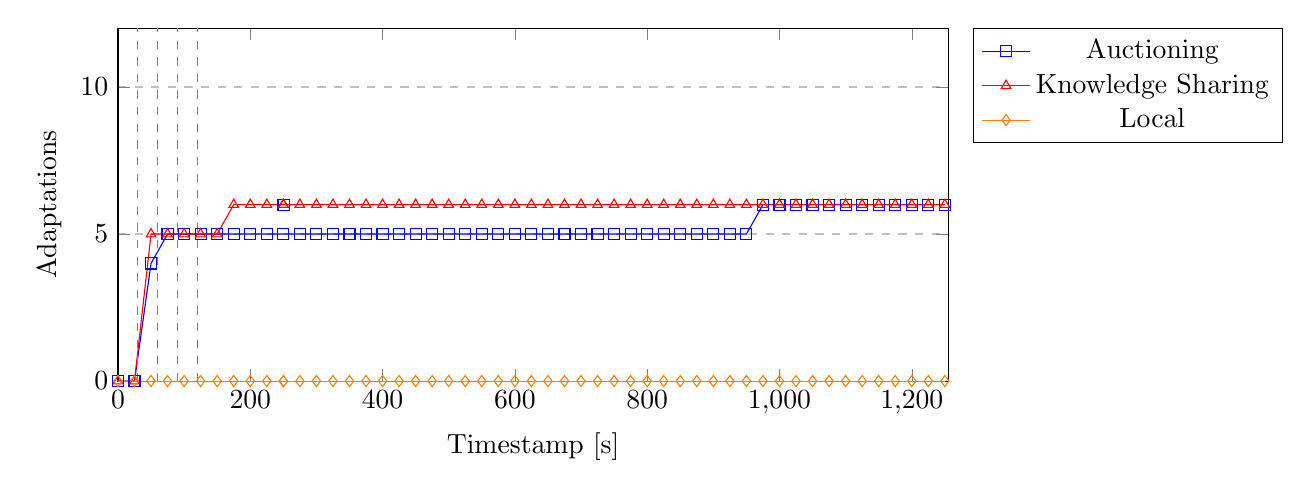
\begin{tikzpicture}
\begin{axis}[
    xlabel={Timestamp [s]},
    ylabel={Adaptations},
    xmin=0, xmax=1255000,
    ymin=0, ymax=12,
    legend pos=outer north east,
    ymajorgrids=true,
    grid style=dashed,
    width=\textwidth,
    height=0.5\textwidth,
    scaled x ticks=base 10:-3,
    xtick scale label code/.code={}
]

	\addplot[color=blue,mark=square] coordinates {
        (0,0)(25000,0)(50000,4)(75000,5)(100000,5)(125000,5)(150000,5)(175000,5)(200000,5)(225000,5)(250000,5)(275000,5)(300000,5)(325000,5)(350000,5)(375000,5)(400000,5)(425000,5)(450000,5)(475000,5)(500000,5)(525000,5)(550000,5)(575000,5)(600000,5)(625000,5)(650000,5)(675000,5)(700000,5)(725000,5)(750000,5)(775000,5)(800000,5)(825000,5)(850000,5)(875000,5)(900000,5)(925000,5)(950000,5)(975000,6)(1000000,6)(1025000,6)(1050000,6)(1075000,6)(1100000,6)(1125000,6)(1150000,6)(1175000,6)(1200000,6)(1225000,6)(1250000,6)(250362,6)
    };
    \addlegendentry{Auctioning}
	\addplot[color=red,mark=triangle] coordinates {
        (0,0)(25000,0)(50000,5)(75000,5)(100000,5)(125000,5)(150000,5)(175000,6)(200000,6)(225000,6)(250000,6)(275000,6)(300000,6)(325000,6)(350000,6)(375000,6)(400000,6)(425000,6)(450000,6)(475000,6)(500000,6)(525000,6)(550000,6)(575000,6)(600000,6)(625000,6)(650000,6)(675000,6)(700000,6)(725000,6)(750000,6)(775000,6)(800000,6)(825000,6)(850000,6)(875000,6)(900000,6)(925000,6)(950000,6)(975000,6)(1000000,6)(1025000,6)(1050000,6)(1075000,6)(1100000,6)(1125000,6)(1150000,6)(1175000,6)(1200000,6)(1225000,6)(1250000,6)(250334,6)
    };
    \addlegendentry{Knowledge Sharing}
	\addplot[color=orange,mark=diamond] coordinates {
        (0,0)(25000,0)(50000,0)(75000,0)(100000,0)(125000,0)(150000,0)(175000,0)(200000,0)(225000,0)(250000,0)(275000,0)(300000,0)(325000,0)(350000,0)(375000,0)(400000,0)(425000,0)(450000,0)(475000,0)(500000,0)(525000,0)(550000,0)(575000,0)(600000,0)(625000,0)(650000,0)(675000,0)(700000,0)(725000,0)(750000,0)(775000,0)(800000,0)(825000,0)(850000,0)(875000,0)(900000,0)(925000,0)(950000,0)(975000,0)(1000000,0)(1025000,0)(1050000,0)(1075000,0)(1100000,0)(1125000,0)(1150000,0)(1175000,0)(1200000,0)(1225000,0)(1250000,0)(250168,0)
    };
    \addlegendentry{Local}

	\addplot[color=gray, dashed,] coordinates {(30000,0) (30000,12)};
	\addplot[color=gray, dashed,] coordinates {(60000,0) (60000,12)};
	\addplot[color=gray, dashed,] coordinates {(90000,0) (90000,12)};
	\addplot[color=gray, dashed,] coordinates {(120000,0) (120000,12)};


\end{axis}
\end{tikzpicture}
    \caption{Graph showing the total amount of adaptations applied by agents in the unstable scenario.}
    \label{fig:proposals-unstable}
\end{figure}

Figure \ref{fig:proposals-unstable} is similar to the \emph{No change} scenario (Figure \ref{fig:proposals-no-change}), and is inline with the damage reduction visible in Figure \ref{fig:overall-damage-unstable}. No new adaptations are applied, and the infrastructure remains stable. The agents also do not detect any new risks, as the properties remain the same. This is reflected in Figure \ref{fig:risk-count-unstable} and \ref{fig:risk-remaining-unstable}.

\begin{figure}[H]
    \centering
        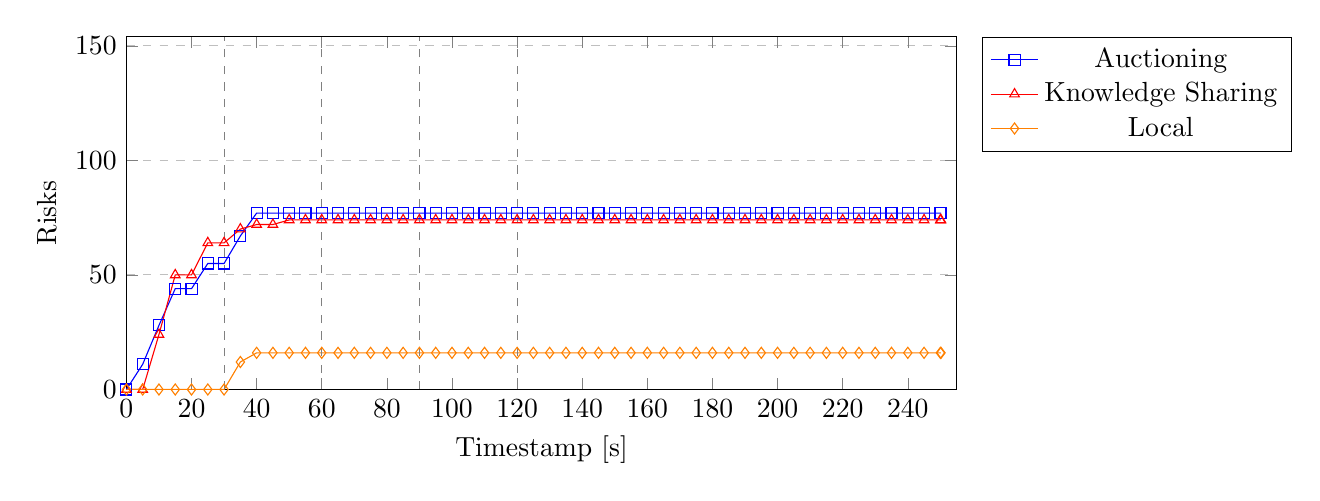
\begin{tikzpicture}
\begin{axis}[
    xlabel={Timestamp [s]},
    ylabel={Risks},
    xmin=0, xmax=255000,
    ymin=0, ymax=154,
    legend pos=outer north east,
    ymajorgrids=true,
    grid style=dashed,
    width=\textwidth,
    height=0.5\textwidth,
    scaled x ticks=base 10:-3,
    xtick scale label code/.code={}
]

	\addplot[color=blue,mark=square] coordinates {
        (0,0)(5000,11)(10000,28)(15000,44)(20000,44)(25000,55)(30000,55)(35000,67)(40000,77)(45000,77)(50000,77)(55000,77)(60000,77)(65000,77)(70000,77)(75000,77)(80000,77)(85000,77)(90000,77)(95000,77)(100000,77)(105000,77)(110000,77)(115000,77)(120000,77)(125000,77)(130000,77)(135000,77)(140000,77)(145000,77)(150000,77)(155000,77)(160000,77)(165000,77)(170000,77)(175000,77)(180000,77)(185000,77)(190000,77)(195000,77)(200000,77)(205000,77)(210000,77)(215000,77)(220000,77)(225000,77)(230000,77)(235000,77)(240000,77)(245000,77)(250000,77)(250270,77)
    };
    \addlegendentry{Auctioning}
	\addplot[color=red,mark=triangle] coordinates {
        (0,0)(5000,0)(10000,24)(15000,50)(20000,50)(25000,64)(30000,64)(35000,70)(40000,72)(45000,72)(50000,74)(55000,74)(60000,74)(65000,74)(70000,74)(75000,74)(80000,74)(85000,74)(90000,74)(95000,74)(100000,74)(105000,74)(110000,74)(115000,74)(120000,74)(125000,74)(130000,74)(135000,74)(140000,74)(145000,74)(150000,74)(155000,74)(160000,74)(165000,74)(170000,74)(175000,74)(180000,74)(185000,74)(190000,74)(195000,74)(200000,74)(205000,74)(210000,74)(215000,74)(220000,74)(225000,74)(230000,74)(235000,74)(240000,74)(245000,74)(250000,74)(250172,74)
    };
    \addlegendentry{Knowledge Sharing}
	\addplot[color=orange,mark=diamond] coordinates {
        (0,0)(5000,0)(10000,0)(15000,0)(20000,0)(25000,0)(30000,0)(35000,12)(40000,16)(45000,16)(50000,16)(55000,16)(60000,16)(65000,16)(70000,16)(75000,16)(80000,16)(85000,16)(90000,16)(95000,16)(100000,16)(105000,16)(110000,16)(115000,16)(120000,16)(125000,16)(130000,16)(135000,16)(140000,16)(145000,16)(150000,16)(155000,16)(160000,16)(165000,16)(170000,16)(175000,16)(180000,16)(185000,16)(190000,16)(195000,16)(200000,16)(205000,16)(210000,16)(215000,16)(220000,16)(225000,16)(230000,16)(235000,16)(240000,16)(245000,16)(250000,16)(250190,16)
    };
    \addlegendentry{Local}

	\addplot[color=gray, dashed,] coordinates {(30000,0) (30000,154)};
	\addplot[color=gray, dashed,] coordinates {(60000,0) (60000,154)};
	\addplot[color=gray, dashed,] coordinates {(90000,0) (90000,154)};
	\addplot[color=gray, dashed,] coordinates {(120000,0) (120000,154)};


\end{axis}
\end{tikzpicture}
    \caption{Graph showing the number of unique risks detected by agents in the unstable scenario.}
    \label{fig:risk-count-unstable}
\end{figure}

\begin{figure}[H]
    \centering
        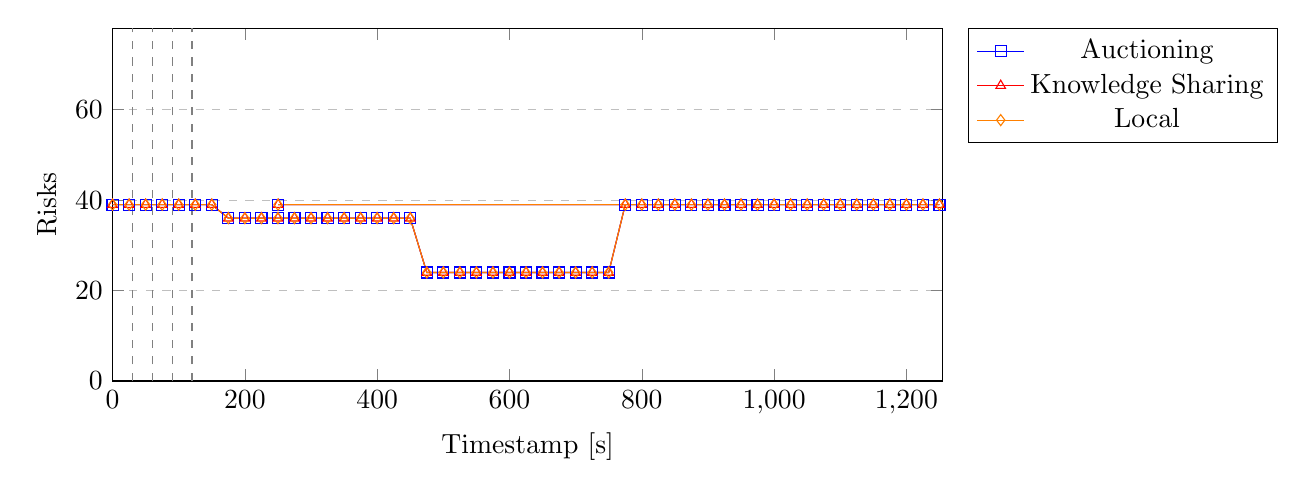
\begin{tikzpicture}
\begin{axis}[
    xlabel={Timestamp [s]},
    ylabel={Risks},
    xmin=0, xmax=1255000,
    ymin=0, ymax=78,
    legend pos=outer north east,
    ymajorgrids=true,
    grid style=dashed,
    width=\textwidth,
    height=0.5\textwidth,
    scaled x ticks=base 10:-3,
    xtick scale label code/.code={}
]

	\addplot[color=blue,mark=square] coordinates {
        (0,39)(25000,39)(50000,39)(75000,39)(100000,39)(125000,39)(150000,39)(175000,36)(200000,36)(225000,36)(250000,36)(275000,36)(300000,36)(325000,36)(350000,36)(375000,36)(400000,36)(425000,36)(450000,36)(475000,24)(500000,24)(525000,24)(550000,24)(575000,24)(600000,24)(625000,24)(650000,24)(675000,24)(700000,24)(725000,24)(750000,24)(775000,39)(800000,39)(825000,39)(850000,39)(875000,39)(900000,39)(925000,39)(950000,39)(975000,39)(1000000,39)(1025000,39)(1050000,39)(1075000,39)(1100000,39)(1125000,39)(1150000,39)(1175000,39)(1200000,39)(1225000,39)(1250000,39)(250362,39)
    };
    \addlegendentry{Auctioning}
	\addplot[color=red,mark=triangle] coordinates {
        (0,39)(25000,39)(50000,39)(75000,39)(100000,39)(125000,39)(150000,39)(175000,36)(200000,36)(225000,36)(250000,36)(275000,36)(300000,36)(325000,36)(350000,36)(375000,36)(400000,36)(425000,36)(450000,36)(475000,24)(500000,24)(525000,24)(550000,24)(575000,24)(600000,24)(625000,24)(650000,24)(675000,24)(700000,24)(725000,24)(750000,24)(775000,39)(800000,39)(825000,39)(850000,39)(875000,39)(900000,39)(925000,39)(950000,39)(975000,39)(1000000,39)(1025000,39)(1050000,39)(1075000,39)(1100000,39)(1125000,39)(1150000,39)(1175000,39)(1200000,39)(1225000,39)(1250000,39)(250334,39)
    };
    \addlegendentry{Knowledge Sharing}
	\addplot[color=orange,mark=diamond] coordinates {
        (0,39)(25000,39)(50000,39)(75000,39)(100000,39)(125000,39)(150000,39)(175000,36)(200000,36)(225000,36)(250000,36)(275000,36)(300000,36)(325000,36)(350000,36)(375000,36)(400000,36)(425000,36)(450000,36)(475000,24)(500000,24)(525000,24)(550000,24)(575000,24)(600000,24)(625000,24)(650000,24)(675000,24)(700000,24)(725000,24)(750000,24)(775000,39)(800000,39)(825000,39)(850000,39)(875000,39)(900000,39)(925000,39)(950000,39)(975000,39)(1000000,39)(1025000,39)(1050000,39)(1075000,39)(1100000,39)(1125000,39)(1150000,39)(1175000,39)(1200000,39)(1225000,39)(1250000,39)(250168,39)
    };
    \addlegendentry{Local}

	\addplot[color=gray, dashed,] coordinates {(30000,0) (30000,78)};
	\addplot[color=gray, dashed,] coordinates {(60000,0) (60000,78)};
	\addplot[color=gray, dashed,] coordinates {(90000,0) (90000,78)};
	\addplot[color=gray, dashed,] coordinates {(120000,0) (120000,78)};


\end{axis}
\end{tikzpicture}
    \caption{Graph showing the number of remaining risks in the infrastructure in the unstable scenario.}
    \label{fig:risk-remaining-unstable}
\end{figure}

\add{write}

\begin{figure}[H]
    \hspace*{-1cm}
    \centering
        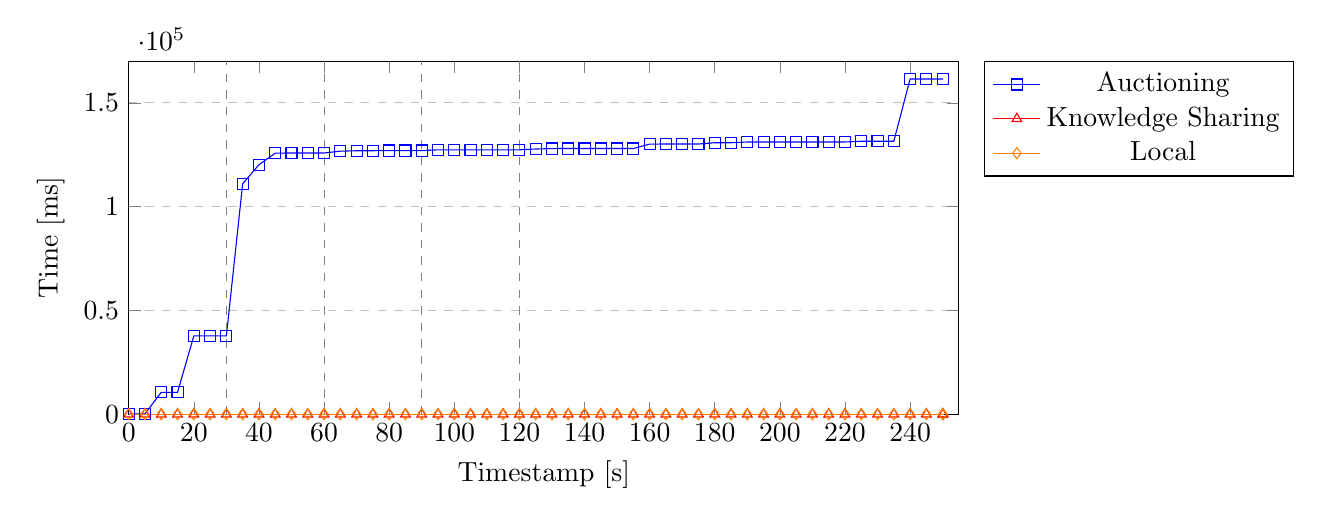
\begin{tikzpicture}
\begin{axis}[
    xlabel={Timestamp [s]},
    ylabel={Time [ms]},
    xmin=0, xmax=255000,
    ymin=0, ymax=170017,
    legend pos=outer north east,
    ymajorgrids=true,
    grid style=dashed,
    width=\textwidth,
    height=0.5\textwidth,
    scaled x ticks=base 10:-3,
    xtick scale label code/.code={}
]

	\addplot[color=blue,mark=square] coordinates {
        (0,0)(5000,173)(10000,10538)(15000,10538)(20000,37730)(25000,37730)(30000,37730)(35000,111030)(40000,120177)(45000,125786)(50000,125855)(55000,125855)(60000,125855)(65000,126731)(70000,126932)(75000,126952)(80000,127013)(85000,127013)(90000,127013)(95000,127365)(100000,127365)(105000,127385)(110000,127385)(115000,127385)(120000,127385)(125000,127764)(130000,127985)(135000,128006)(140000,128006)(145000,128006)(150000,128006)(155000,128006)(160000,130144)(165000,130172)(170000,130172)(175000,130172)(180000,130795)(185000,130795)(190000,131135)(195000,131135)(200000,131161)(205000,131161)(210000,131161)(215000,131161)(220000,131161)(225000,131489)(230000,131517)(235000,131517)(240000,161517)(245000,161517)(250000,161517)(250144,161517)
    };
    \addlegendentry{Auctioning}
	\addplot[color=red,mark=triangle] coordinates {
        (0,0)(5000,0)(10000,0)(15000,0)(20000,0)(25000,0)(30000,0)(35000,0)(40000,0)(45000,0)(50000,0)(55000,0)(60000,0)(65000,0)(70000,0)(75000,0)(80000,0)(85000,0)(90000,0)(95000,0)(100000,0)(105000,0)(110000,0)(115000,0)(120000,0)(125000,0)(130000,0)(135000,0)(140000,0)(145000,0)(150000,0)(155000,0)(160000,0)(165000,0)(170000,0)(175000,0)(180000,0)(185000,0)(190000,0)(195000,0)(200000,0)(205000,0)(210000,0)(215000,0)(220000,0)(225000,0)(230000,0)(235000,0)(240000,0)(245000,0)(250000,0)(250118,0)
    };
    \addlegendentry{Knowledge Sharing}
	\addplot[color=orange,mark=diamond] coordinates {
        (0,0)(5000,0)(10000,0)(15000,0)(20000,0)(25000,0)(30000,0)(35000,0)(40000,0)(45000,0)(50000,0)(55000,0)(60000,0)(65000,0)(70000,0)(75000,0)(80000,0)(85000,0)(90000,0)(95000,0)(100000,0)(105000,0)(110000,0)(115000,0)(120000,0)(125000,0)(130000,0)(135000,0)(140000,0)(145000,0)(150000,0)(155000,0)(160000,0)(165000,0)(170000,0)(175000,0)(180000,0)(185000,0)(190000,0)(195000,0)(200000,0)(205000,0)(210000,0)(215000,0)(220000,0)(225000,0)(230000,0)(235000,0)(240000,0)(245000,0)(250000,0)(250091,0)
    };
    \addlegendentry{Local}

	\addplot[color=gray, dashed,] coordinates {(30000,0) (30000,170017)};
	\addplot[color=gray, dashed,] coordinates {(60000,0) (60000,170017)};
	\addplot[color=gray, dashed,] coordinates {(90000,0) (90000,170017)};
	\addplot[color=gray, dashed,] coordinates {(120000,0) (120000,170017)};


\end{axis}
\end{tikzpicture}
    \caption{Graph showing the sum of time spent auctioning by agents in the unstable scenario.}
    \label{fig:auctioning-time-unstable}
\end{figure}

\begin{figure}[H]
    \hspace*{-1cm}
    \centering
        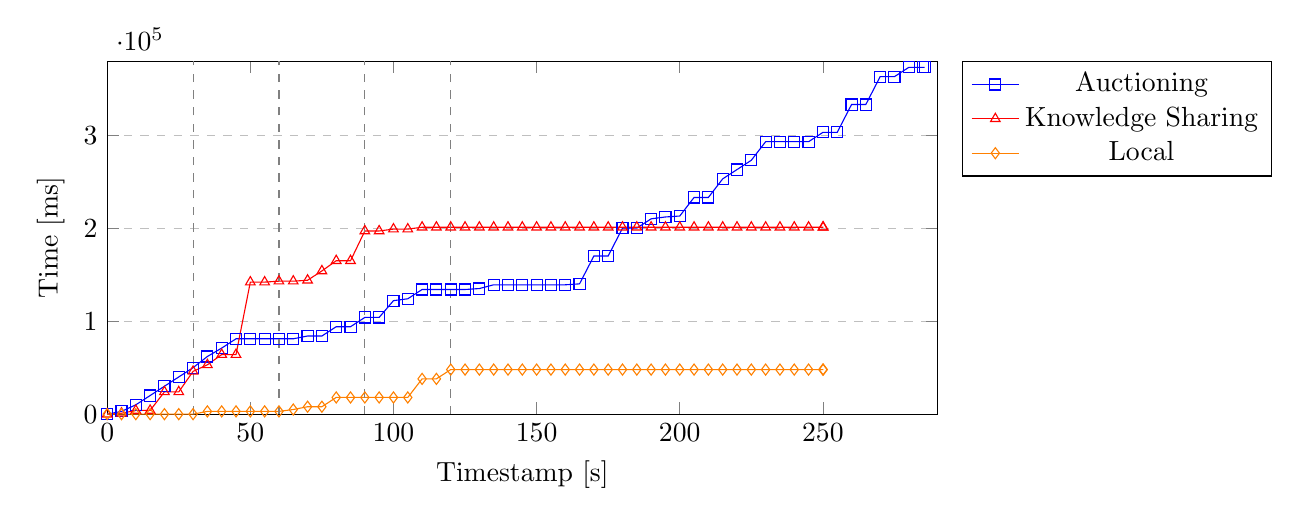
\begin{tikzpicture}
\begin{axis}[
    xlabel={Timestamp [s]},
    ylabel={Time [ms]},
    xmin=0, xmax=290000,
    ymin=0, ymax=380038,
    legend pos=outer north east,
    ymajorgrids=true,
    grid style=dashed,
    width=\textwidth,
    height=0.5\textwidth,
    scaled x ticks=base 10:-3,
    xtick scale label code/.code={}
]

	\addplot[color=blue,mark=square] coordinates {
        (0,0)(5000,3015)(10000,10073)(15000,20083)(20000,30092)(25000,40100)(30000,50105)(35000,62134)(40000,71193)(45000,81199)(50000,81199)(55000,81199)(60000,81199)(65000,81199)(70000,84209)(75000,84209)(80000,94219)(85000,94219)(90000,104222)(95000,104222)(100000,122281)(105000,124295)(110000,134306)(115000,134306)(120000,134306)(125000,134306)(130000,135314)(135000,139351)(140000,139351)(145000,139351)(150000,139351)(155000,139351)(160000,139351)(165000,140360)(170000,170377)(175000,170377)(180000,200396)(185000,200396)(190000,210405)(195000,212415)(200000,213423)(205000,233437)(210000,233437)(215000,253455)(220000,263466)(225000,273475)(230000,293490)(235000,293490)(240000,293490)(245000,293490)(250000,303496)(255000,303496)(260000,333521)(265000,333521)(270000,363542)(275000,363542)(280000,373547)(285000,373547)(285530,373547)
    };
    \addlegendentry{Auctioning}
	\addplot[color=red,mark=triangle] coordinates {
        (0,0)(5000,1009)(10000,4030)(15000,4030)(20000,24044)(25000,24044)(30000,46078)(35000,53188)(40000,64205)(45000,64205)(50000,142255)(55000,142255)(60000,143258)(65000,143258)(70000,144266)(75000,154274)(80000,165289)(85000,165289)(90000,197316)(95000,197316)(100000,199335)(105000,199335)(110000,201346)(115000,201346)(120000,201346)(125000,201346)(130000,201346)(135000,201346)(140000,201346)(145000,201346)(150000,201346)(155000,201346)(160000,201346)(165000,201346)(170000,201346)(175000,201346)(180000,201346)(185000,201346)(190000,201346)(195000,201346)(200000,201346)(205000,201346)(210000,201346)(215000,201346)(220000,201346)(225000,201346)(230000,201346)(235000,201346)(240000,201346)(245000,201346)(250000,201346)(250138,201346)
    };
    \addlegendentry{Knowledge Sharing}
	\addplot[color=orange,mark=diamond] coordinates {
        (0,0)(5000,0)(10000,0)(15000,0)(20000,0)(25000,0)(30000,0)(35000,3011)(40000,3011)(45000,3011)(50000,3011)(55000,3011)(60000,3011)(65000,5019)(70000,8033)(75000,8033)(80000,18038)(85000,18038)(90000,18038)(95000,18038)(100000,18038)(105000,18038)(110000,38043)(115000,38043)(120000,48045)(125000,48045)(130000,48045)(135000,48045)(140000,48045)(145000,48045)(150000,48045)(155000,48045)(160000,48045)(165000,48045)(170000,48045)(175000,48045)(180000,48045)(185000,48045)(190000,48045)(195000,48045)(200000,48045)(205000,48045)(210000,48045)(215000,48045)(220000,48045)(225000,48045)(230000,48045)(235000,48045)(240000,48045)(245000,48045)(250000,48045)(250134,48045)
    };
    \addlegendentry{Local}

	\addplot[color=gray, dashed,] coordinates {(30000,0) (30000,380038)};
	\addplot[color=gray, dashed,] coordinates {(60000,0) (60000,380038)};
	\addplot[color=gray, dashed,] coordinates {(90000,0) (90000,380038)};
	\addplot[color=gray, dashed,] coordinates {(120000,0) (120000,380038)};


\end{axis}
\end{tikzpicture}
    \caption{Graph showing the sum of time spent adapting by agents in the unstable scenario.}
    \label{fig:adapting-time-unstable}
\end{figure}

As with the prior graphs for this scenario we see that Figure \ref{fig:adapting-time-unstable} is also stable after the first $50$ seconds. There are no new risks as shown in Figure \ref{fig:risk-count-unstable} and no new adaptations are necessary to mitigate them. 
